\chapter{Literature Review}

In the United States, the study of the frame-based SLU started in the 1970’s in the DARPA
Speech Understanding Research (SUR) and then the Resource Management (RM) tasks. At
this early stage, natural language understanding (NLU) techniques like finite state machine
(FSM) and augmented transition networks (ATNs) were applied for SLU \cite{d1e535}. The
study of SLU surged in the 90’s, with the DARPA sponsored Air Travel Information System
(ATIS) evaluations \cite{dahl}. Multiple research labs from both
academia and industry, including AT\&T, BBN, Carnegie Mellon University, MIT and SRI,
developed systems that attempted to understand users’ spontaneous spoken queries for air
travel information (including flight information, ground transportation information, airport
service information, etc.) and then obtain the answers from a standard database. ATIS is an important milestone for the frame-based SLU, largely thanks to its rigorous componentwise
and end-to-end evaluation, participated by multiple institutions, with a common test set.

\begin{figure}[h]
	\centering
	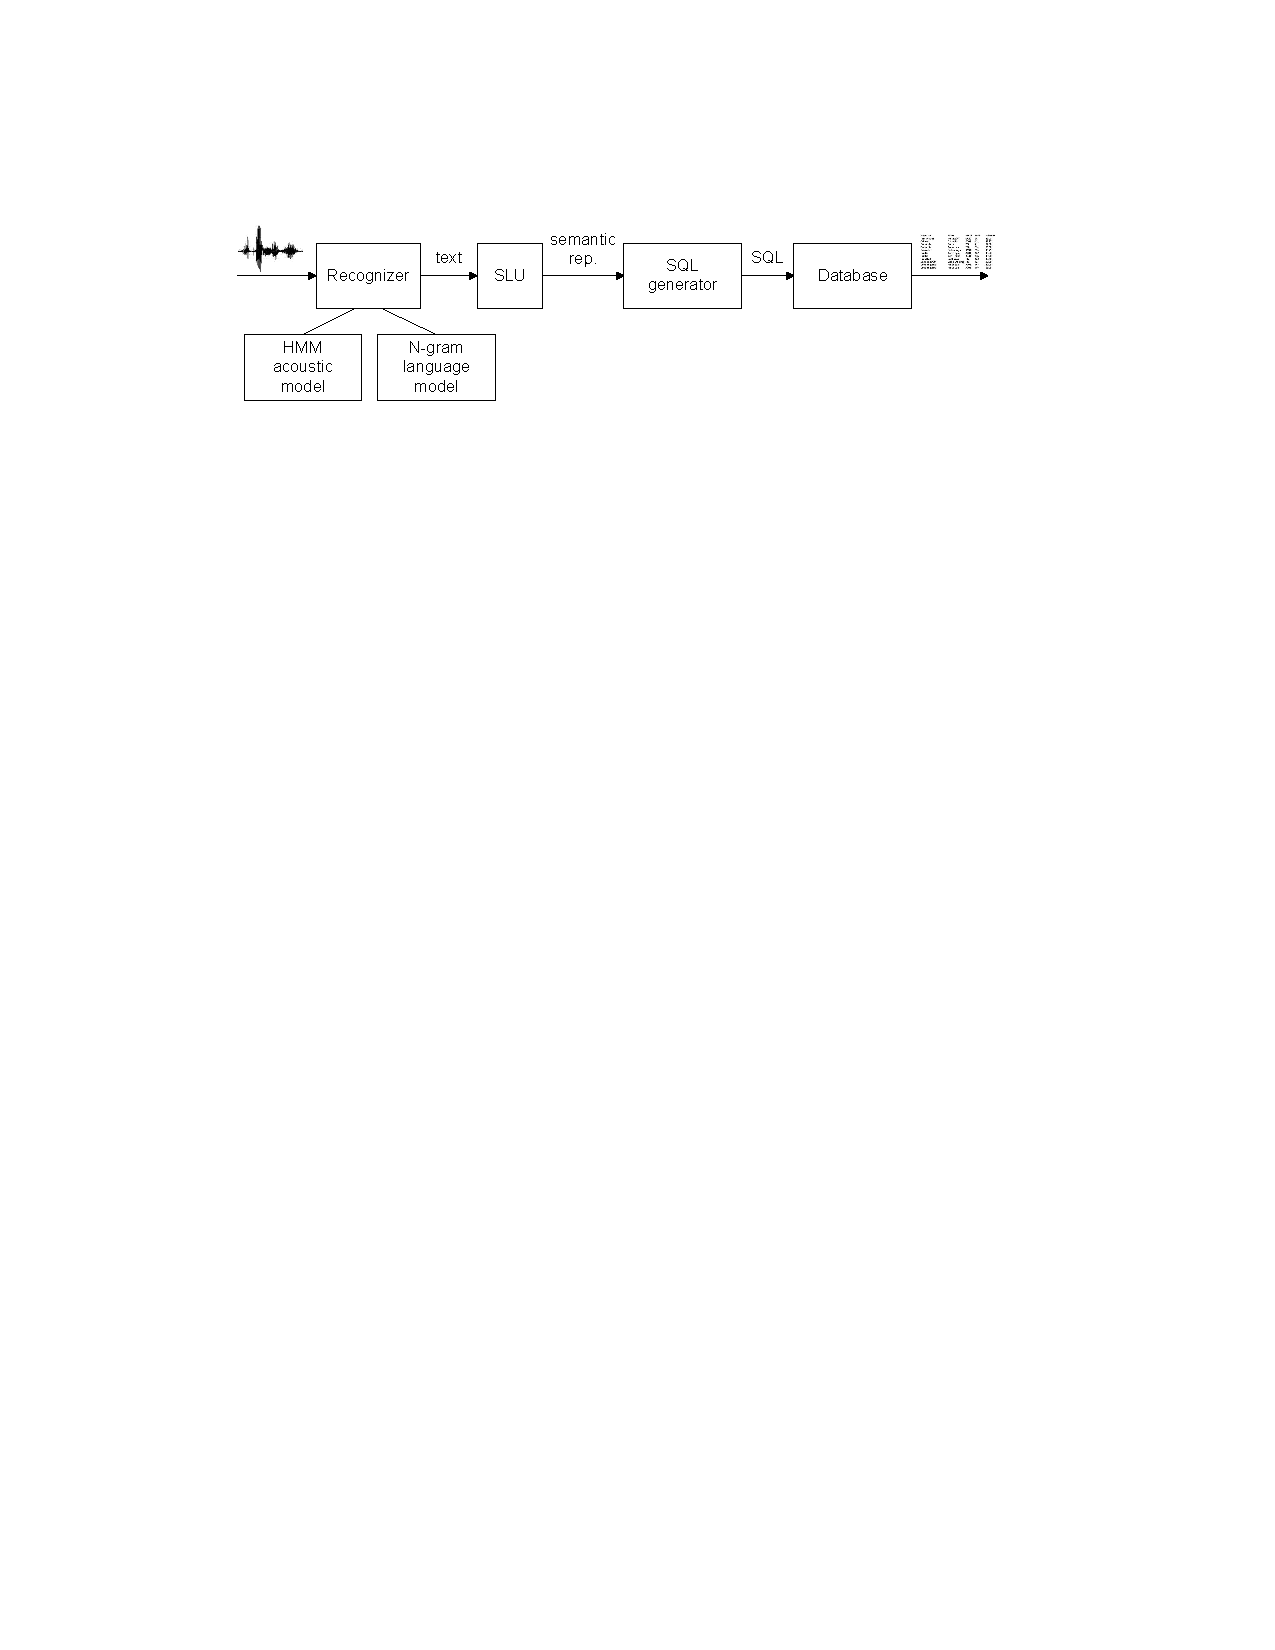
\includegraphics[width=\textwidth]{fig/atis-seq}
\caption[Frame based SLU in a typical ATIS system]{Frame-based SLU in a typical ATIS system, which consists of 1) a speech recognizer with both the acoustic model and language model trained with the ATIS specific data; 2) a SLU system that extracts the semantic representation (meaning) from the recognized text; and 3) a SQL generator that automatically generates the database query based on the semantic representation.}
\end{figure}


Figure 2.1 shows the role of the frame-based SLU component in a typical ATIS system.
While ATIS focused more or less on the understanding of a single-turn utterance, the
more recent DARPA Communicator program \cite{d1e358} focused on the rapid and
cost-effective development of multi-modal speech enabled dialog systems, in which general
infrastructures for dialog systems were developed, where different component systems for
ASR, SLU, DM and TTS can be plugged in and evaluated. Naturally, many SLU technologies
developed in ATIS were used in the SLU component of the Communicator program. Eight
systems from AT\&T, BBN, University of Colorado, Carnegie Mellon University, IBM,
Lucent Bell Labs, MIT, and SRI participated in the 2001 evaluation \cite{d1e411}.
In the mean time, the AI community had separate effort in building a conversational planning
agent, such as the TRAINS system \cite{d1e5}.

Parallel efforts were made on the other side of the Atlantic. The French EVALDA/MEDIA
project aimed at designing and testing the evaluation methodology to compare and
diagnose the context-dependent and independent SLU capability in spoken language dialogs.
Participants included both academic organizations (IRIT, LIA, LIMSI, LORIA, VALORIA,
CLIPS) and industrial institutions (FRANCE TELECOM R\&D, TELIP). Like ATIS, the
domain of this study was restricted to database queries for tourist and hotel information.

The more recent LUNA project sponsored by the European Union focused on the
problem of real-time understanding of spontaneous speech in the context of advanced
telecom services. Its major objective is the development of a robust SLU toolkit for dialog
systems, which enhances users experience by allowing natural human-machine interactions
via spontaneous and unconstrained speech. One special characteristic of the project, which
is absent in the similar projects in the US, is its emphasis on multilingual portability of the
SLU components.

\section{Technical Challenges}
The frame-based SLU is closely related to natural language understanding (NLU), a field
that has been studied for more than half a century. NLU focus mainly on understanding
of general domain written texts. Because there is not a specific application domain for the
general purposed NLU, the semantics in NLU have to be defined in a broader sense, such
as thematic roles (agents, patients, etc.) In contrast, the frame-based SLU has, in the current
state of technology, focused only on specific application domains. The semantics are defined
very specifically according to the application domain, as illustrated by the above examples
of semantic frames. Many domain-specific constraints can be included in the understanding
model. Ostensibly, this may make the problem easier to solve. Unfortunately, there are many
new challenges for spoken language understanding, including
\begin{itemize}
\item Extra-grammaticality – spoken languages are not as well-formed as written
languages. People are in general less careful with speech than with writings. They
often do not comply with rigid syntactic constraints.
\item Disfluencies – false starts, repairs, and hesitations are pervasive, especially in
conversational speech.
\item Speech recognition errors – Speech recognition technologies are far from perfect.
Environment noise, speaker’s accent, domain specific terminologies, all make speech
recognition errors inevitable. It is common to see that a generic speech recognizer has
over 30\% word error rates on domain specific data.
\item Out-of-domain utterances – a dialog system can never restrict a user from saying
anything out of a specific domain, even in a system-initiated dialog, where users are
prompted for answers to specific questions. Because the frame-based SLU focuses on
a specific application domain, out-of-domain utterances are not well modeled and can
often be confused as an in-domain utterance. Detecting the out-of-domain utterances is
not an easy task – it is complicated by the extra-grammaticality, disfluencies and ASR
errors of in-domain utterances.
\end{itemize}

\section{Knowledge Based Solutions}
\subsection{Semantically Enhanced Syntactic Grammar}
Many advocates of the knowledge-based approach believe that general linguistic knowledge
is helpful in modeling domain specific language. This includes the syntactic constraints
as well as some optional rudimentary domain-independent semantic knowledge. However,
since the ultimate goal is to extract the domain-dependent semantic information, one major
question is how to inject the domain specific semantic constraints into a domain-independent
grammar.

MIT’s TINA system \cite{d1e333} aims at the graceful, seamless interface between syntax
and semantics. It uses context free grammar (augmented with a set of features used to enforce several syntactic and semantic constraints via unification). The injection of the domain-dependent semantics is accomplished by replacing the low level syntactic nonterminals
with the semantic non-terminals. In doing so, the top level syntactic rules makes
the grammar capable of modeling the domain-independent linguistic constraints, such as
the Wh-movement/trace-management.

SRI’s Gemini system \cite{d1e149} is implemented on top of its Core Language
Engine (CLE) \cite{d1e35}, a general natural language understanding system that parses
an input sentence and generates its semantic representation in the logical forms. Here the
unification grammar is also used to model the general syntactic constraints. Unlike TINA
that blends syntax and semantics together with the mixed grammar categories in constituent
parsing, it clearly separates the domain independent syntax from the domain dependent
semantics. Another specialty of Gemini is its adoption of the logical forms instead of the
frame-like representation for semantics.

\subsection{Semantic Grammars}
While using the semantically-enhanced syntactic grammars saves grammar developers from
the effort to model the general language structures, it requires profound knowledge about the
general syntactic grammars. In addition, the knowledge-based approach often requires the
exact matching of input sentences to the grammar rules, which makes it not robust to ASR
errors, extra-grammaticality and disfluencies in spontaneous speech. Often it has to resort to
some kind of semantic-based robust parsing as a backup.

The Phoenix spoken language understanding system \cite{d1e509} directly models the
domain dependent semantics with a semantic grammar. It was used by CMU in the ATIS
evaluation, and was one of the top performing SLU systems in the evaluation. As we have
discussed previously about semantic representation, it uses semantic frames to represent
semantic relations – the basic type of action for the application. Slots in a frame are filled by
matching the input strings (sentences) against the slot-nets, the recursive transition networks
(RTNs) that specifies the patterns for filler strings. RTNs are finite state transition networks,
where the arcs in the networks can include not only terminal words, but also calls to other
networks. They are equivalents of the context free grammars in graph representation.

\section{Data Driven Approaches}
The knowledge-based solution has the advantage of not requiring much labeled data. In
addition, almost everyone can start writing a SLU grammar with some basic training. The
grammar can be used as both the ASR language model and the SLU model in a single pass
speech understanding. However, a knowledge-based system is difficulty and expensive to
develop and maintain due to the following reasons:

1. Grammar development is an error-prone process. While it does not take much effort for
a common developer to learn the syntax for writing a speech understanding grammar,
it requires combined linguistic and engineering expertises, plus the deep knowledge
about the application domain, to write a good grammar. Grammar authoring is a
balancing act between simplicity and coverage. People talk differently, therefore a
good grammar has to account for the different expressions for the same concept, action
or request. If a grammar is too simple, it is inadequate to model the linguistic diversity.
On the other hand, if a grammar is too complicated, it may not only slow down the
parser, but also increase the ambiguities, hence confuses the SLU system and degrades
its performance. Design the structure of a grammar is an art. It takes much experience
to have a good design where frequently used concepts, for example, are modeled by
separate rules to be shared by other rules at a higher level.

2. It takes multiple rounds to fine tune a grammar. Grammar authoring can hardly be a
one-shot deal – nobody can write a perfect grammar with a single try. Furthermore,
grammars need to evolve over time – new features and scenarios may be introduced
to an application after its initial deployment. Ideally, an SLU system should be
able to automatically adapt to the real data collected after its deployment. On the
contrary, knowledge-based systems require an expert’s involvement, sometimes even
the involvement of the original system designer, in the adaptation loop.

3. Grammar authoring is difficult to scale up. It is relatively easy to write a grammar
to model a single concept as in a system-initiated dialog system, where the user
is prompted to provide a single piece of information (e.g., name, account number,
social security number, address, etc.) at a dialog turn. However, if we allow users to
volunteer multiple pieces of information in a single utterance, the ways to put together
these pieces are combinational. As we have shown previously, for a very restricted
domain like ATIS, the semantic grammar already contains 3.2k non-terminals and 13k
grammar rules.

SLU based on data-driven statistical learning approaches directly addresses many of
the problems associated with the knowledge-based solutions. Statistical SLU systems can
automatically learn from example sentences with their corresponding semantics annotated.
Compared to the manual grammar authoring, the annotations are much easier to create,
without the requirement of the specialized knowledge. The statistical approach can adapt
to new data, possibly via unsupervised learning. One disadvantage of such an approach,
however, is the data-sparseness problem. The requirement of a large amount of labeled
training data is not very practical in real-world applications, which are quite different from a
few showcase problems studied in research labs. This is the case especially at the early stage
of system development.

\subsection{Generative Models}
In the statistical frame-based SLU, the task is often formalized as a pattern recognition
problem. Given the word sequence W, the goal of SLU is to find the semantic representation
of the meaning M that has the maximum a posteriori probability $P(M|W)$.
And the objective function of a generative model is to maximize the joint probability
$P(W, M) = P(W | M)P(M)$ given a training sample of W and its semantic annotation
M.

Two separate models exist in this generative framework. The semantic prior model $P(M)$
assigns probability to an underlying semantic structure or meaning M. The lexicalization
model $P(W | M)$, sometimes called lexical generation or realization model \cite{d1e218}, assigns probability to the surface sentence (i.e., word/lexical sequence) W given the
semantic structure.

\subsubsection{Semantic Priors in Understanding Models}
In statistical SLU that models cross-word contextual dependency, each state represents
a slot in a semantic frame. For the systems that use the flat concepts for semantic
representation, such as AT\&T’s CHRONUS \cite{d1e252} and IBM’s fertility
model \cite{d1e114}, the topology of the model is a fully connected network.
For models that use hierarchical semantic structures, including BBN’s Hidden
Understanding Model \cite{d1e218} and Microsoft Research’s HMM/CFG composite
model \cite{d1e473}, the semantic prior is a natural extension.

Cambridge University’s Hidden Vector State model \cite{dataset-flickr30k} uses another way
to model the semantic prior with hierarchical structures. Named the hidden vector states, the
states in the Markov chain represent the stack status of the pre-terminal nodes (the nodes
immediately above the terminal words) in a semantic tree. The hidden vector states encode all the structure information about the tree, so the semantic tree structure (without the terminal words) can be reconstructed from the hidden vector state sequence. The model imposes a hard limit on the maximum depth of the stack, so the number of the states becomes finite, and the prior model becomes the Markov chain in an HMM.

\subsubsection{Lexicalisation Models}
The first lexicalization model, used by both CHRONUS and
the Hidden Understanding Model, assumes a deterministic one-to-one
correspondence between model states and the segments, i.e., there is only one segment per
state, and the order of the segments follows the order of the states.

\cite{d1e193} introduces a 2+1 SLU model that integrates the normalization process in
the lexicalization model. Here the number “2” stands for the semantic prior model and the
concept model, which is the traditional lexicalization model that generates the lexical string
from the concept. “1” stands for the additional model that treat the normalized attribute
values as a hidden variables.

\subsubsection{Implementation of Generative Models}
Many generative models are implemented with standard toolkits like the stochastic finite
state transducers (SFST) \cite{raymond} or the graphic models \cite{d1e56}. For example, each SLU component can be implemented as a SFST, and the
SLU system can be built by composing the component SFSTs. Raymond and Riccardi
(2007) shows a SFST implementation of a generative model. The lattice from an ASR
is represented by a stochastic finite state machine (SFSM) λW . It uses an n-gram as the
lexicalization model for “concepts”, which are slots or a null attribute that models the carrier
phrases connecting the slots. N-gram can be represented by a SFSM as well, as described
in \cite{d1e301}. An n-gram SFSM for a concept can be turned into a SFST by
outputting the accepted words together with the concept’s name. The union of all the SFSTs
for all concepts forms the lexicalization model λw2c that maps words to concepts. Finally, a
statistical conceptual language model is used as the semantic prior model. The SFST model
λCLM is flexible enough to implemented different semantic prior models.

The generative models can also be easily implemented with the general purpose graphic
model toolkit. For example, researchers from Universit´e d’Avignon used Dynamic Bayesian
Networks (DBNs) \cite{d1e193} to implement generative SLU models.

\subsection{Integrated Models}
One disadvantage of a purely data-driven, statistical SLU approach is the requirement
of a large amount of training data. The preprocessing step is not modeled statistically as an integral part of the SLU model. The lack of information about the preprocessing model makes the statistical SLU model unable to predict the words for speech recognition, and it prohibits the model from properly normalizing the probabilities because the actual length of the segment replaced by the superword is unknown to the SLU model. An HMM/CFG composite lexicalization model has been introduced in \cite{wang2006}, which we review here, to aim at solving these problems. This model uses the same semantic prior for hierarchical Markov topology. The underlying state corresponding to a slot in the semantic frame is expanded into a preamble-filler-postamble three state sequence. The preamble and postamble serve as the contextual clue for the identity of the
slot, while the slot filler decides its value. The lexicalization model follows similar
to CHRONUS and the Hidden Understanding model. 

The HMM/CFG composite model balances the trade-off between robustness and
the constraints on over-generalizations/ambiguities with the different models for the
preambles/postambles and the slot fillers. The CFG model imposes a relatively rigid
restriction on the slot fillers, which are more crucial for correct understanding and less
subject to the disfluencies because they are semantically coherent units. The fillers are often
domain specific and can be obtained from the application database, like the city names and
airport names in the ATIS domain; or they are common domain-independent concepts like
phone number, date, time, which are already modeled in a grammar library; or they can be
automatically generated according to some high level description like a regular expression
for an alphanumeric concept \cite{wang2006}. The non-slot states serve as the “glue”
that sticks different slot fillers together. This type of inter-concept language is normally
domain dependent, hard to pre-build a model for, and subject to more disfluencies. It varies
significantly across different speakers. The n-gram model is more robust and thus suitable
for this sub-language. Furthermore, the knowledge introduced by the CFG sub-model greatly
compensates for the data sparseness problem (e.g., it is very unlikely to see all city names
occur in all context in the training data).

\subsection{Conditional Models}
The statistical models for SLU we have introduced so far are all generative models – the
semantic structure M is first generated according to the semantic prior model $P(M)$, from
which the observation W is generated according to $P(W | M)$, which an be modeled by the
different lexicalization processes we just described.

Conditional models are non-generative. In a conditional model, the states (which encode
the meaning M) are directly conditioned on the observation. For SLU, Conditional Random
Fields (CRFs) or Hidden State Conditional Random Fields (HCRFs) are commonly used
conditional models. With CRFs or HCRFs, the conditional probability of the entire state
(label) sequence y given the observation sequence is modeled as an exponential (log-linear)
distribution, with respect to a set of features $f(y, x)$.

\cite{wang2006} compared the use of CRF, perceptron,
large margin, and MCE using stochastic gradient descent (SGD) for
SF in the ATIS domain. They obtained significantly reduced slot error
rates, with best performance achieved by CRF (though it was the
slowest to train).

Almost simultaneously \cite{dataset-flickr30k} proposed the use of
CRF, extended by non-local features, which are important to disambiguate
the type of the slot. For example, a day can be the arrival
day, departure day, or the return day. If the contextual cues disambiguating
them are beyond the immediate context, it is not easy for
the classifier to choose the correct class. Using non-local trigger
features automatically extracted from the training data is shown to
improve the performance significantly.

Finally, \cite{raymond} compared SVM and CRF
with generative models for the ATIS task. They concluded that discriminative
methods perform significantly better, and furthermore, it
is possible to incorporate a-priori information or long distance features
easily. For example they added features such as “Does this
utterance have the verb arrive”. This resulted in about 10\% relative
reduction in slot error rate. The design of such features usually
requires domain knowledge.

\subsection{Neural Models}
In comparison to the above described techniques, deep
learning uses many layers of neural networks. It has made
strong impacts on applications ranging from automatic speech
recognition to image recognition.

A distinguishing feature of NLP applications of deep learning
is that inputs are symbols from a large vocabulary, which led
the initial work on neural language modeling to suggest
map words to a learned distributed representation either in the
input or output layers (or both), with those embeddings learned
jointly with the task. Following this principle, a variety of neural
net architectures and training approaches have been successfully
applied. Particularly, RNNs are also widely used in NLP. One can represent an input symbol
as a one-hot vector, i.e., containing zeros except for one component
equal to one, and this weight vector is considered as a
low-dimensional continuous valued vector representation of the
original input, called word embedding. Critically, in this vector
space, similar words that have occurred syntactically and semantically
tend to be placed by the learning procedure close
to each other, and relationships between words are preserved.
Thus, adjusting the model parameters to increase the objective
function for a training example which involves a particular
word tends to improve performances for similar words in
similar context, thereby greatly improving generalization and
addressing the curse-of-dimensionality obstacle faced with traditional
n-gram non-parametric models [26].

Recently, RNNs \cite{multijoint} and convoluational \cite{cnn} neural networks
(CNNs) have been applied to SLU. The Elman \cite{elman1990finding} architecture
adopted in uses past hidden activities, together
with the observations, as the input to the same hidden layer,
which in turn applies a nonlinear transformation to convert
the inputs to activities. The Jordan architecture exploited
in uses past predictions at the output layer instead of the
past hidden activities as additional inputs to the hidden layer.
CNNs are used similar to that in to extract features
through convolving and pooling operations. CNNs achieved
comparable performances to RNNs on SLU tasks.

The RNNs in are trained to optimize the frame
cross-entropy criterion. More recently, sequence discriminative
training is used to train RNNs. Similar work is
conducted for CNNs. The main motivation of using
sequence discriminative training is to overcome the label
biasness problem that is addressed by CRFs. It incorporates
dependence between output tags and adds a knowledge
source for performance improvements.